\documentclass[aspectratio=169%可调屏宽比16:9(169),4:3(43)
,serif,mathserif]{beamer}
\mode<presentation>{
%\usetheme{default}
%\usetheme{AnnArbor}
%\usetheme{Antibes}
%\usetheme{Bergen}
%\usetheme{Berkeley}
%\usetheme{Berlin}
%\usetheme{Boadilla}
%\usetheme{CambridgeUS}
%\usetheme{Copenhagen}
%\usetheme{Darmstadt}
%\usetheme{Dresden}
%\usetheme{Frankfurt}
%\usetheme{Goettingen}
%\usetheme{Hannover}
%\usetheme{Ilmenau}
%\usetheme{JuanLesPins}
%\usetheme{Luebeck}
\usetheme{Madrid}
%\usetheme{Malmoe}
%\usetheme{Marburg}
%\usetheme{Montpellier}
%\usetheme{PaloAlto}
%\usetheme{Pittsburgh}
%\usetheme{Rochester}
%\usetheme{Singapore}
%\usetheme{Szeged}
%\usetheme{Warsaw}
% As well as themes, the Beamer class has a number of color themes
% for any slide theme. Uncomment each of these in turn to see how it
% changes the colors of your current slide theme.
%\usecolortheme{albatross}
%\usecolortheme{beaver}
%\usecolortheme{beetle}
%\usecolortheme{crane}
%\usecolortheme{dolphin}
%\usecolortheme{dove}
%\usecolortheme{fly}
%\usecolortheme{lily}
%\usecolortheme{orchid}
%\usecolortheme{rose}
%\usecolortheme{seagull}
%\usecolortheme{seahorse}
%\usecolortheme{whale}
%\usecolortheme{wolverine}
%\setbeamertemplate{footline} % To remove the footer line in all slides uncomment this line
%\setbeamertemplate{footline}[page number] % To replace the footer line in all slides with a simple slide count uncomment this line
%\setbeamertemplate{navigation symbols}{} % To remove the navigation symbols from the bottom of all slides uncomment this line
}
\usepackage{adjustbox}
\usepackage{indentfirst} 
\usepackage{amsmath, amsfonts, epsfig, xspace}
\usepackage{algorithm,algorithmic}
\usepackage{beamerthemesplit}
\usepackage{booktabs}
\usepackage{bm}
\usepackage{braket}
\usepackage{calligra}
\usepackage[T1]{fontenc}
\usepackage{fontspec}
\usepackage{ctex}
\usepackage{latexsym}
\usepackage{multicol}
\usepackage{multimedia}
\usepackage{calligra} \DeclareMathAlphabet{\mathcalligra}{T1}{calligra}{m}{n} \DeclareFontShape{T1}{calligra}{m}{n}{<->s*[2.2]callig15}{}
\usepackage{pstricks,pst-node}
\usepackage{ragged2e}
\usepackage{setspace}
\usepackage[normal,tight,center]{subfigure}
\setlength{\subfigcapskip}{-.5em}
\setlength{\parindent}{2em}
\begin{document}
\title{A programming model of verification of neural network } % The short title appears at the bottom of every slide, the full title is only on the title page
\author[Chi~Zhiming]{迟智名} % Your name
\institute[ISCAS] % Your institution as it will appear on the bottom of every slide, may be shorthand to save space
{	
	%Lanzhou University \\ % Your institution for the title page
	%\medskip
	%\textit{chizhm16@lzu.edu.cn} % Your email address
}
	\CTEXoptions[today=old]
	\date{\today} % Date, can be changed to a custom date
\begin{frame}[plain]\vspace{1.5em}
\titlepage\vspace{-0.5cm}
%\centerline{\includegraphics[height=0.30\textheight]{logo.png}}
%\hfill 指导教师:xxx
\end{frame}
\begin{frame}{目录}
\tableofcontents
\end{frame}
\AtBeginSection[]
{
\begin{frame}{\tiny}
\frametitle{目录}
\tableofcontents[currentsection]
\end{frame}
}
%----------------------------------------------------------------------------------------
%	PRESENTATION SLIDES
%----------------------------------------------------------------------------------------

%------------------------------------------------
\section{Introduction} % Sections can be created in order to organize your presentation into discrete blocks, all sections and subsections are automatically printed in the table of contents as an overview of the talk
%------------------------------------------------

\begin{frame}
	\frametitle{Reference paper}
	\begin{itemize}
		\item Integrating Simplex with DPLL(T)
		\item Reluplex: An Efficient SMT Solver for Verifying Deep Neural Networks
	\end{itemize}
\end{frame}

\begin{frame}
	\frametitle{Neural network model}
	\begin{columns}
		\begin{column}{.6\textwidth}
			\begin{figure}[htbp]
				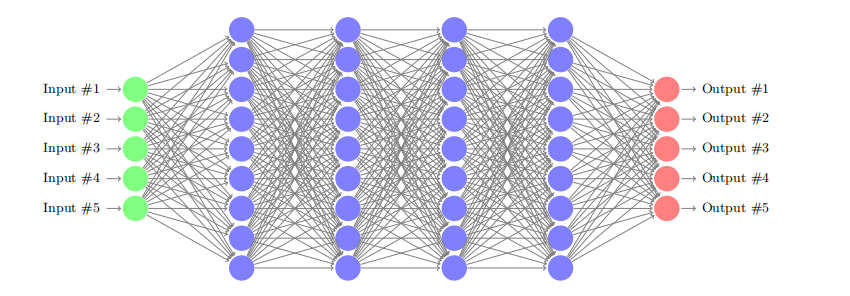
\includegraphics[width=1\linewidth]{1.png}
			\end{figure}
		\end{column}

		\begin{column}{.4\textwidth}
			\begin{itemize}
				\item $s_i$: the size of layer $i$.
				\item $v_{i,j}$: The value of the j-th node of layer i.
				\item $V_i$: the column vector $[v_{i,1}, . . . , v_{i,si} ]$.
				\item Relu(x): max(0,x)
				\item $V_i = ReLU(W_iV_{i−1} + B_i), W_i: s_i \times s_{i-1},B_i: s_i$
			\end{itemize}
		\end{column}
	\end{columns}

\end{frame}

\section{Programming model}
\begin{frame}
	\frametitle{verification of neural network}
	A small example: 
	\begin{columns}
		\begin{column}{.65\textwidth}
			\begin{figure}[htbp]
				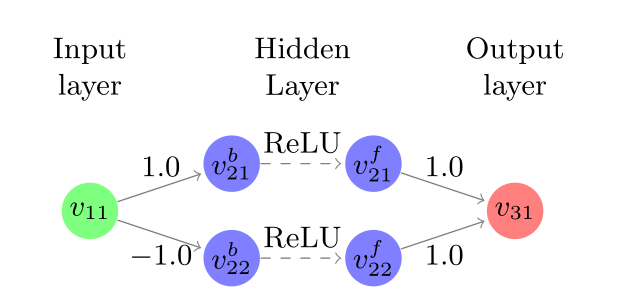
\includegraphics[width=1\linewidth]{4.png}
			\end{figure}
		\end{column}

		\begin{column}{.35\textwidth}
			To verify Property:
			\begin{itemize}
				\item $v_{11} \in [0,1] $
				\item $v_{31} \in [0.5,1] $
			\end{itemize}
		\end{column}
	\end{columns}
\end{frame}

\begin{frame}
	\frametitle{Programming model}
	\begin{columns}
		\begin{column}{.5\textwidth}
			\begin{figure}[htbp]
				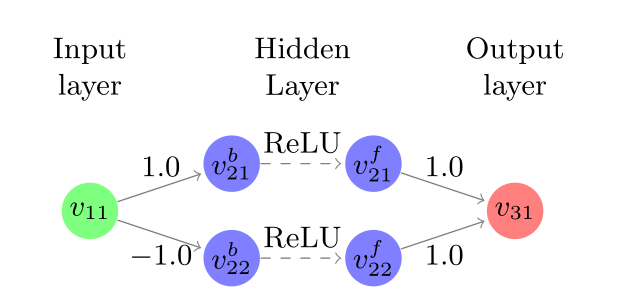
\includegraphics[width=1\linewidth]{4.png}
			\end{figure}
		\end{column}

		\begin{column}{.5\textwidth}
			To verify Property:
			\begin{itemize}
				\item Verify: $v_{11} \in[0,1] \text { and } v_{31} \in[0.5,1]$
				\item equation constraints:
				\begin{equation}
					\left\{
						\begin{array}{lll}
						& a_{1}=-v_{11}+v_{21}^{b} \\
						& a_{2}=v_{11}+v_{22}^{b} \\
						& a_{3}=-v_{21}^{f}-v_{22}^{f}+v_{31} \\
					\end{array} \right.
				\end{equation}
				\item bound constraints: 
				\begin{equation}
					\left\{
						\begin{array}{lll}
						& a_{1,2,3}= 0 \\
						& v_{21}^{b},v_{22}^{b} \in (-\infty,\infty)\\
						& v_{21}^{f},v_{22}^{f} \in (0,\infty)\\
					\end{array} \right.
				\end{equation}
			\end{itemize}
		\end{column}
	\end{columns}
\end{frame}


\begin{frame}
	\frametitle{Programming model}
	\begin{columns}
		\begin{column}{.5\textwidth}
			\begin{figure}[htbp]
				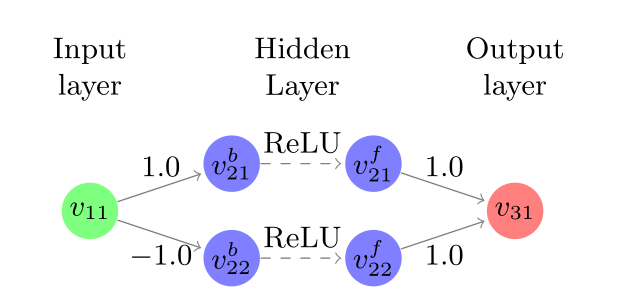
\includegraphics[width=1\linewidth]{4.png}
			\end{figure}
		\end{column}

		\begin{column}{.5\textwidth}
			Split constraints:
			\begin{itemize}
				\item $(v_{21}^{b} \geq 0 \implies v_{21}^{f} = v_{21}^{b}) \wedge (v_{21}^{b} \leq 0 \implies v_{21}^{f} = 0) $
				\item $(v_{22}^{b} \geq 0 \implies v_{22}^{f} = v_{22}^{b}) \wedge (v_{22}^{b} \leq 0 \implies v_{22}^{f} = 0) $
			\end{itemize}
		\end{column}
	\end{columns}
\end{frame}

\begin{frame}
	\frametitle{Programming model}
	\begin{itemize}
		\item equation constraints:
		\begin{equation}
			\left\{
				\begin{array}{lll}
				& a_{1}=-v_{11}+v_{21}^{b} \\
				& a_{2}=v_{11}+v_{22}^{b} \\
				& a_{3}=-v_{21}^{f}-v_{22}^{f}+v_{31} \\
			\end{array} \right.
		\end{equation}
		\item bound constraints:
		\begin{equation}
			\left\{
				\begin{array}{lll}
				& v_{11} \in[0,1],v_{31} \in[0.5,1] \\
				& a_{1,2,3}= 0 \\
				& v_{21}^{b},v_{22}^{b} \in (-\infty,\infty)\\
				& v_{21}^{f},v_{22}^{f} \in (0,\infty)\\
			\end{array} \right.
		\end{equation}
		\item Split constraints:
		\begin{equation}
			\left\{
				\begin{array}{lll}
				& (v_{21}^{b} \geq 0 \implies v_{21}^{f} = v_{21}^{b}) \wedge (v_{21}^{b} \leq 0 \implies v_{21}^{f} = 0)\\
				& (v_{22}^{b} \geq 0 \implies v_{22}^{f} = v_{22}^{b}) \wedge (v_{22}^{b} \leq 0 \implies v_{22}^{f} = 0) \\
			\end{array} \right.
		\end{equation}
	\end{itemize}
\end{frame}

\begin{frame}
	\frametitle{Discussion: NPC-problem}
	\begin{itemize}
		\item Note the split constraints:
		\begin{equation}
			\left\{
				\begin{array}{lll}
				& (v_{21}^{b} \geq 0 \implies v_{21}^{f} = v_{21}^{b}) \wedge (v_{21}^{b} \leq 0 \implies v_{21}^{f} = 0)\\
				& (v_{22}^{b} \geq 0 \implies v_{22}^{f} = v_{22}^{b}) \wedge (v_{22}^{b} \leq 0 \implies v_{22}^{f} = 0) \\
			\end{array} \right.
		\end{equation}
		\item n nodes $\to 2^n$ conditions
		\item this theoretical worst-case behavior is also seen in practice	
	\end{itemize}
\end{frame}


\section{An actual instance:ACAS Xu}
\begin{frame}
	\frametitle{ACAS Xu(Airborne Collision Avoidance System X unmanned)}
	\begin{columns}
		\begin{column}{.6\textwidth}
			\begin{figure}
				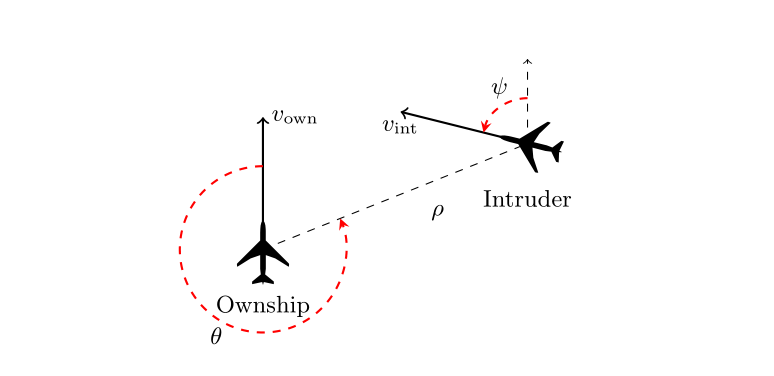
\includegraphics[width=0.75\linewidth]{12.png}
			\end{figure}
		\end{column}

		\begin{column}{.4\textwidth}			
			\begin{itemize}
				\item Input of networks: $v_{own},v_{int},p,\theta,\phi$
				\item 45 networks: 5 previous advisories multiplies 9 discretizing(Time until loss of vertical separation)
				\item 5 outputs: SL,SR,WL,WR,COC(Clear-of-Conflict)
			\end{itemize}
		\end{column}
	\end{columns}

\end{frame}

\begin{frame}
	\frametitle{Prove Network Properties}
	\begin{figure}
		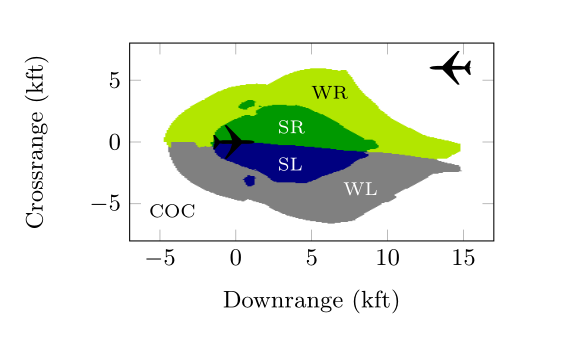
\includegraphics[width=0.75\linewidth]{13.png}
	\end{figure}

	% \begin{itemize}
	% 	\item The system does not give unnecessary turning advisories
	% 	\item Alerting regions are uniform and do not contain inconsistent alerts
	% 	\item Strong alerts do not appear for high vertical separation values.
	% \end{itemize}
\end{frame}

%------------------------------------------------


%------------------------------------------------

%------------------------------------------------


%------------------------------------------------
\begin{frame}
\hfill
\center{\Huge{\calligra{\Huge{Thank you}}}}
\linespread{3}\selectfont
\end{frame}
%----------------------------------------------------------------------------------------
\end{document}